\section{Evaluation}
\label{sec:eval}

Our application, in addition to implementing our WiFi policies, would send a UDP packet stamped with a sequence number to a server every 100 milliseconds. To evaluate the performance of our policies, we performed several experiments, both with and without the policies enabled. For each experiment, we inspected which packets were received to determine how many packets were dropped, and for how long Internet connectivity was lost.

We present the setup and results from two experiments here. They were designed to address the second and third problem situations presented, connecting to a network requiring authentication and remaining connected to a weak network respectively. In order to test the internet access testing policy, we aproached a store with complimentary WiFi, requireing authentication. For predictive WiFi abandonment, we tested on a WiFi network that was known to one of the authors to cause clingly WiFi behavior.

\subsection{Internet Access Testing - The Panera Test}
It is inherently difficult to objectively test the problem presented by WiFi networks requiring authentication. The duration of disconnection varies depending on the users' habits and the time spent within range of the network. For example, some users might spend only 2 minutes connected to unusable WiFi before they realize they have to authenticate; other users might take 10 or 30 minutes. Therefore, to best demonstrate this issue, as well as our solution, we opted to test a realistic scenario that we believe represents a potential user experience.

The mobile device and user began the experiment across the street from an establishment with authentication-requiring WiFi. It pinged a server on the Internet via its cellular data network. The user approached the building, and the phone connected to WiFi when it felt that the signal was sufficiently strong. Upon arriving at the door, the user waited for 30 seconds and then attempted to access umich.edu, and waited 10 seconds after successfully loading the page (not including any delay from loading and accepting the terms and conditions).

\begin{figure}
	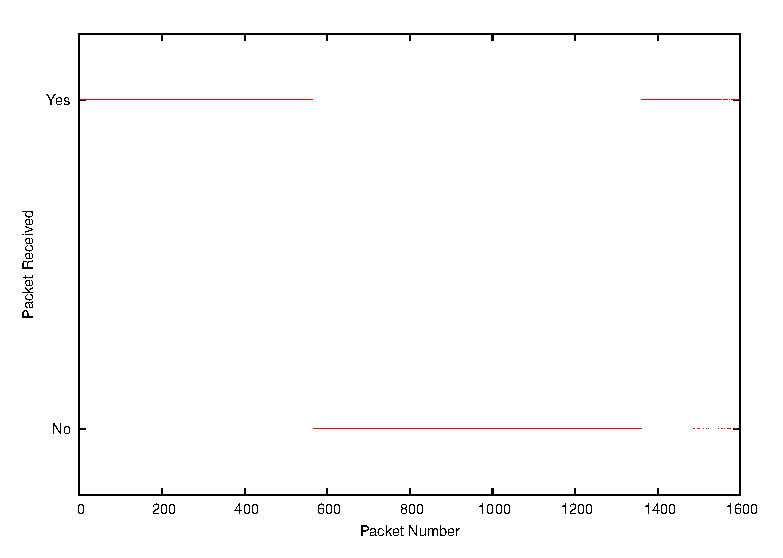
\includegraphics[width=0.5\textwidth]{paneraNoPolicy}
	\caption{TODO}
\end{figure}

Figure 2 shows, as expected, that we did not successfully send a single packet from the time we walked within range of the WiFi network to the time we attempted to access google.com and accepted the establishment's terms and conditions. If a user were to leave his/her phone in his/her pocket - rather than checking it as impulsively as the authors - he/she may never notice that the phone has connected to unusable WiFi. In this case, the user would not receive any incoming data until he/she left the establishment.

When run with Bouncer, the ping recieved a 302 HTTP response (a redirect to the establishment's terms and conditions page) after attempting to reach umich.edu. As per the implemented Bouncer policy, the phone then disconnected and reverted to the cellular data network. Figure 3 shows our drastically reduced downtime. It is worth noting that the limited downtime exists only because our implementation prevents us from checking a WiFi connection's Internet access before Android tears down the cellular connection. Ideally, the network would be tested, and the device would decide to remain on the cellular network, never connecting to WiFi and resulting in no downtime.

While not tested explicitly, we believe that Bouncer could also be applied to the first issue we presented, of connecting to a network, too weak to reach the internet. Receiving an error response would be treated the same as the redirect in this experiment and multiple tests would help identify fleeting connections, such as those possible when passing a building.

\begin{figure}
	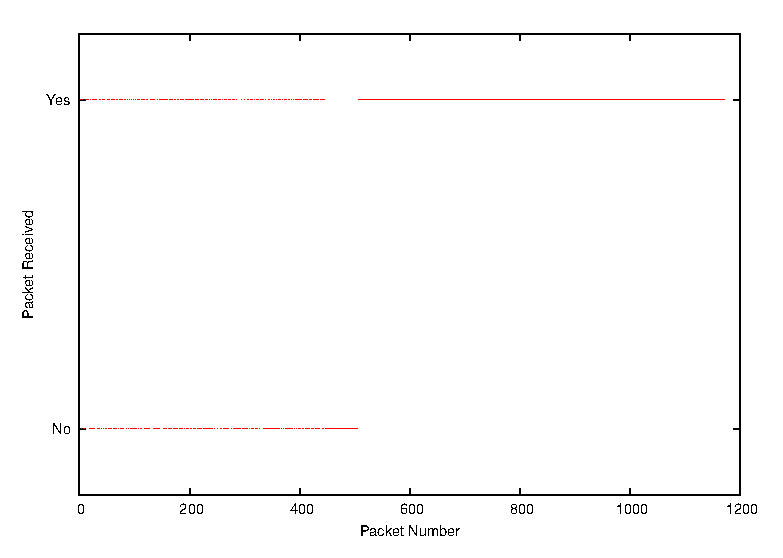
\includegraphics[width=0.5\textwidth]{paneraWithPolicy}
	\caption{TODO}
\end{figure}

\subsection{Predictive WiFi Abandonment - The Courtyards Test}
In order to evaluate our predictive WiFi abandonment policy, the device was tested using a WiFi network with which the authors have experienced disconnection ``clinginess" issues. From a starting position near a WiFi access point (an Apple Airport Express), connected to WiFi, the user took a set route, leaving the range of the network. The route took the device well out of the range of the access point, testing the transition from WiFi to cellular data.

The stock policy resulted in clinging to the WiFi network, at the perimeter of the network's range, where there was little to no connectivity. As seen in figure 4, a substantial number of packets were dropped before the device transitioned to the cellular connection. Another burst of packets are lost shortly after, when the phone tries to reconnect to the network it just left. This demonstrates a pattern the authors experienced which interrupts streaming content, and provides a generally poor user experience.

\begin{figure}
	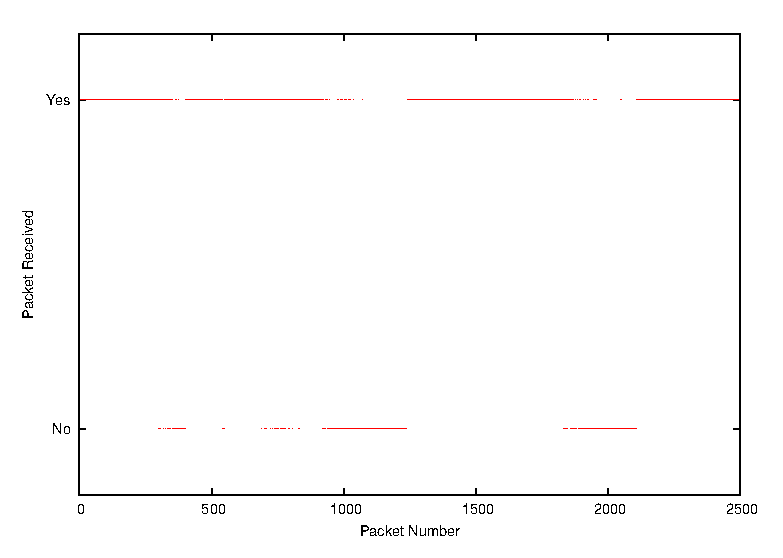
\includegraphics[width=0.5\textwidth]{leavingCourtyardsNoPolicy}
	\caption{TODO}
\end{figure}

When run with the Abandon Ship policy, as demonstrated by figure 5, the phone disconnects much more promptly from WiFi. It then stays on the cellular network, maintaining a stable connection. This more decisive policy does not attempt to stay connected to a WiFi network it should have given up on, resulting in better uptime.

\begin{figure}
	\includegraphics[width=0.5\textwidth]{leavingCourtyardsWithPolicy}
	\caption{TODO}
\end{figure}

\begin{figure}
	\includegraphics[width=0.5\textwidth]{bars}
	\caption{TODO}
\end{figure}
